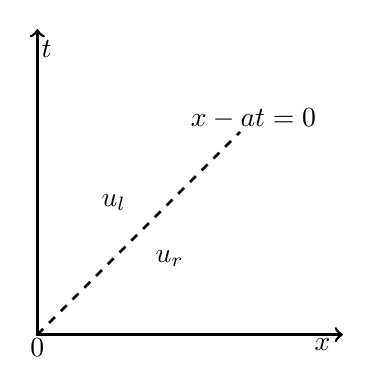
\begin{tikzpicture}[scale = {0.015\linewidth},inner sep = 1pt]
%% \begin{tikzpicture}[scale = {0.015\linewidth},inner sep = 1pt]
%% \tikzstyle{every node} = [draw,circle,fill=gray!30];
%% \draw (-1.5,0.0) circle (0.8);
%% \draw[<->,line width=1pt] (0,1) node[right]{\;$t$}|-(1,0) node[below]{$m$};

\draw[line width=1pt] (0.0,0.7) node[right]{$t$}|-(0.7,0) node[below]{$x$};
\draw[->,line width=1pt] (0.7,0)--(0.75,0);
\draw[->,line width=1pt] (0.0,0.7)--(0.0,0.75);

\node[draw=white] (char) at (0.53033,0.53033) {$x - at = 0$};
\draw[dashed,line width=1pt] (0,0) node[below]{$0$} -- (char); 

\node[draw=white] at (0.18750,0.32476) {$u_l$};
\node[draw=white] at (0.32476,0.18750) {$u_r$};

\end{tikzpicture}
